\documentclass{beamer}
\usepackage[english]{babel}
\usepackage[utf8]{inputenc}
\usepackage{amsmath,amssymb,physics,mathtools,blindtext,graphicx,float}
\usepackage[labelfont=bf]{caption}
\date{}
\title{Mass and radius of white dwarfs and neutron stars}


\begin{document}
\frame{\titlepage}

\begin{frame}
\frametitle{Hydrostatic equilibrium}
\begin{itemize}
    \item The inward force of gravity is balanced by the outward force of pressure.
\end{itemize}
\begin{equation*}
    \vcenter{\hbox{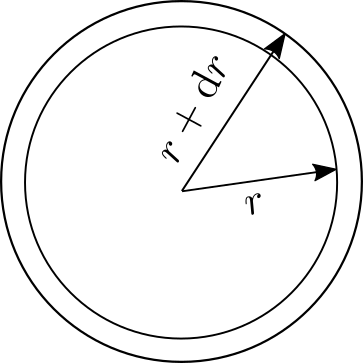
\includegraphics[width=2.3cm,height=2.3cm]{Shell.png}}}
    \qquad\qquad
    \begin{aligned}
        &4\pi r^2\text{d}P = -\frac{GM\cdot \text{d}M}{r^2}\\    
        &\text{d}M = 4\pi r^2\rho(r)\text{d}r
    \end{aligned}
\end{equation*}
\begin{itemize}
    \item This leads to the hydrostatic equations:
    \begin{equation*}
        \begin{split}
            &\frac{\text{d}P}{\text{d}r} = -\frac{GM\rho}{r^2} \\ 
            &\frac{\text{d}M}{\text{d}r} = 4\pi r^2\rho
        \end{split}
    \end{equation*}
    \item The radius of the star $R$ is given by $P(R)=0$ and the mass is $M(R)$.
    \item For very dense stars, relativistic effects have to be taken into account.
\end{itemize}
\end{frame}

\begin{frame}
\frametitle{Tolman-Oppenheimer-Volkoff (TOV) equations}
\begin{itemize}
    \item The TOV-equations are obtained from general relativity when a static and spherically symmetric mass distribution is inserted into the Einstein equations.
    \item The hydrostatic equations above are modified:
    \item[]
\end{itemize}
\begin{equation*}
    \begin{split}
        &\frac{\text{d}P}{\text{d}r} = -\frac{G\left[P+\mathcal{E}(r)\right]\left[M(r)+4\pi r^3P/c^2\right]}{c^2r^2[1-2GM(r)/(c^2r)]} \\ 
        &\frac{\text{d}M}{\text{d}r} = 4\pi r^2\frac{\mathcal{E}(r)}{c^2}
    \end{split}
\end{equation*}
\begin{itemize}
    \item[] where $\mathcal{E} = \rho c^2$.
\end{itemize}
\end{frame}

%\begin{frame}
%\frametitle{Interpretation of TOV-equations}
%\textit{First equation}:
%\begin{equation*}
%    4\pi r^2\text{d}P = -\frac{GM\cdot\text{d}M}{r^2}\left(1+\frac{P}{\mathcal{E}}\right)\left(1+\frac{4\pi r^3P}{Mc^2}\right)\left(1-\frac{2GM}{c^2r}\right)^{-1}
%\end{equation*}
%\begin{itemize}
%    \item The left hand side is the net force acting on a shell lying between radii $r$ and $r+\text{d}r$.
%    \item First factor on right hand side is the attractive Newtonian gravity acting on the shell. 
%    \item The other factors are general relativistic corrections to the Newtonian gravity.
%\end{itemize}
%\textit{Second equation}:
%\begin{equation*}
%    \text{d}M = 4\pi r^2\mathcal{E}\text{d}r/c^2
%\end{equation*}
%\begin{itemize}
%    \item $\text{d}M$ is the gravitational mass of the shell.
%\end{itemize}
%\end{frame}


\begin{frame}
\frametitle{The equation of state (EOS)}
\begin{itemize}
    \item In order to solve the TOV equations, a relation between the energy density $\mathcal{E}$ and the pressure $P$ is needed. 
    \item The function $\mathcal{E}(P)$ is called the equation of state.
    %\item For a degenerate gas of noninteracting neutrons of mass $m_n$, the pressure and energy density can be found as function of number density $n$:
    \begin{equation*}
        \begin{split}
            &\text{White dwarf} \to \text{Degenerate electron gas among inert heavy}\\ 
            &\hspace{2.6cm}\text{nuclei (oxygen and carbon)}. \\ 
            &\text{Neutron star} \to \text{Degenerate neutron gas}.
        \end{split}
    \end{equation*}
\end{itemize}
%\begin{equation*}
%    \begin{split}
%        &\mathcal{E}(n) = \mathcal{E}_0\left(x_F\sqrt{1+x_F^2}\left(1+2x_F^2\right)-\ln\left(x_F+\sqrt{1+x_F^2}\right)\right) \\ 
%        &P(n) = \mathcal{E}_0\left(\frac{2}{3}x_F^3\sqrt{1+x_F^2}-x_F\sqrt{1+x_F^2}+\ln\left(x_F+\sqrt{1+x_F^2}\right)\right)
%    \end{split}
%\end{equation*}
%where 
%\begin{equation*}
%    x_F(n) = \frac{\hbar c(3\pi^2n)^{1/3}}{m_nc^2} \quad \text{and} \quad \mathcal{E}_0 = \frac{(m_nc^2)^4}{8\pi^2(\hbar c)^3}.
%\end{equation*}
\end{frame}

\begin{frame}
\begin{itemize}
    \item \textit{White dwarf}:
    \begin{equation*}
        \begin{split}
            &\mathcal{E}(x) = \left(\frac{m_p}{m_e}\frac{(m_ec^2)^4}{(\hbar c)^3}\right)x^3 + \frac{(m_ec^2)^4}{8\pi^2(\hbar c)^3}F(x) \\ 
            &P(x) = \frac{(m_ec^2)^4}{8\pi^2(\hbar c)^3}G(x)
        \end{split}
    \end{equation*}
    \item \textit{Neutron star}:
    \begin{equation*}
        \begin{split}
            &\mathcal{E}(x) = \frac{(m_nc^2)^4}{8\pi^2(\hbar c)^3}F(x) \\ 
            &P(x) = \frac{(m_nc^2)^4}{8\pi^2(\hbar c)^3}G(x)
        \end{split}
    \end{equation*}
    \item[] where
    \begin{equation*}
        \begin{split}
        &F(x) = x\sqrt{1+x^2}(1+2x^2)-\ln\left(x+\sqrt{1+x^2}\right) \\ 
        &G(x) = \frac{2}{3}x^2\sqrt{1+x^2}-x\sqrt{1+x^2}+\ln\left(x+\sqrt{1+x^2}\right) \\ 
        \end{split}
    \end{equation*}
\end{itemize}
\end{frame}

\begin{frame}
\frametitle{Solving the TOV-equations}
\begin{itemize}
    \item The initial conditions $P_{j=0} = P(0) = P_c$ and $M_{j=0} = M(0) = 0$ were inserted.
    \item The numerical solution was then obtained by finding the the energy density $\mathcal{E}_j$ from $P_j$ using the bisection method and then integrating the system of equations using Heun's method:
\end{itemize}
\begin{center}
    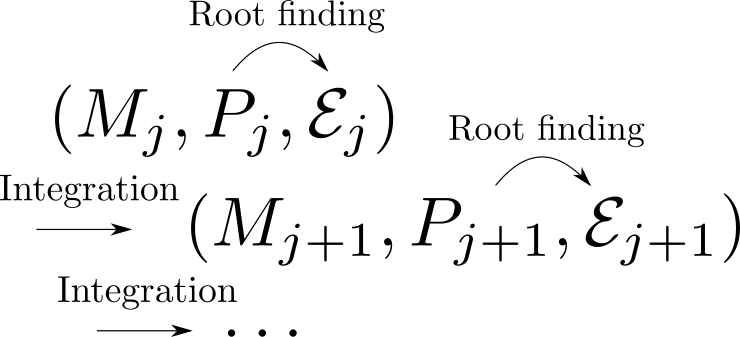
\includegraphics[scale=0.35]{Numerical_scheme.png}
\end{center}
\begin{itemize}
    \item This is repeated until the pressure beomes zero, $P(R) = 0$.
\end{itemize}
\end{frame}

\begin{frame}
\frametitle{Results}
\begin{itemize}
    \item Example with $P_c = P(0) = 0.2$ GeV/fm$^3$:
\end{itemize}
\begin{center}
    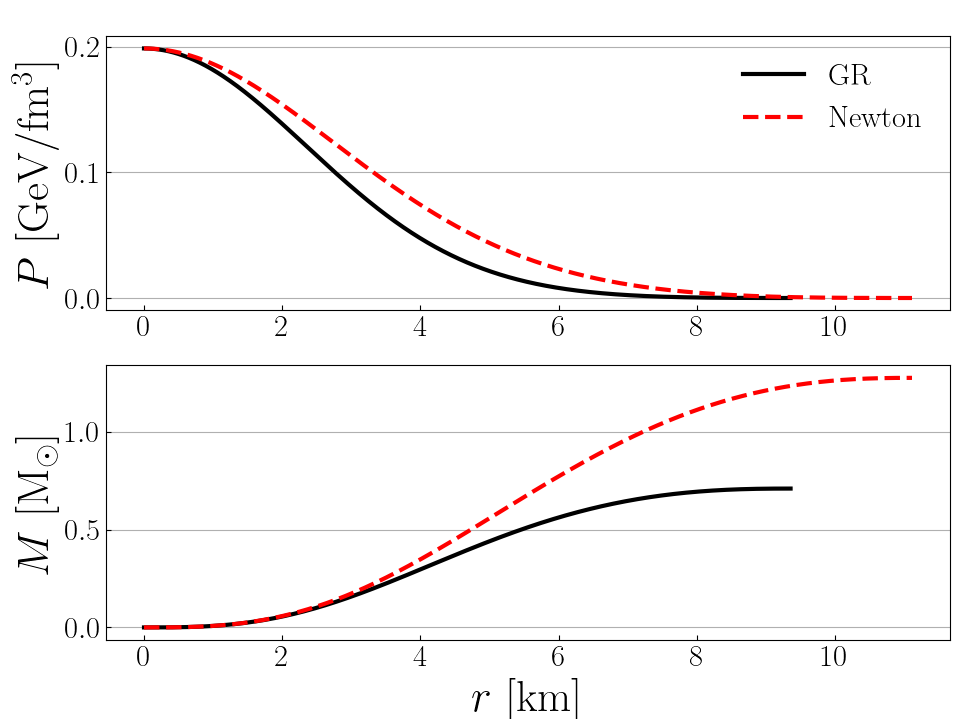
\includegraphics[scale=0.4]{Newt.png}
\end{center}
\end{frame}

\begin{frame}
\frametitle{Results}
\begin{itemize}
    \item Examining the mass and radius for many values of $P_c$:
\end{itemize}
\begin{center}
    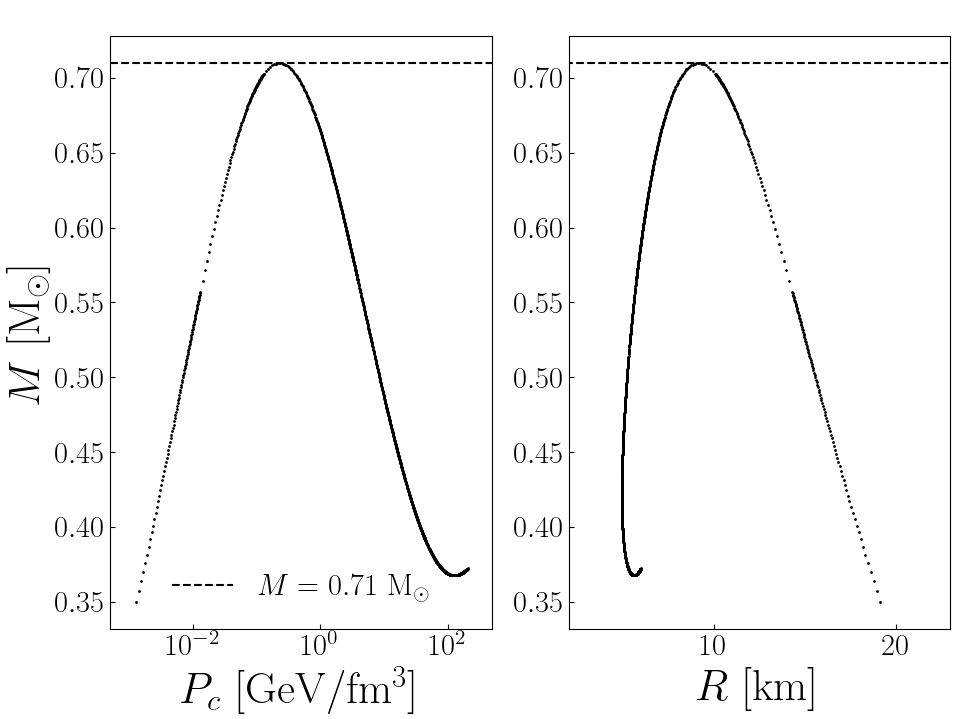
\includegraphics[scale=0.4]{TOV_limit.png}
\end{center}
\end{frame}


\end{document}
